\documentclass{article}

\usepackage{amsmath}
\usepackage{amsfonts}
\usepackage{graphicx}
\usepackage[section]{placeins}
\usepackage[a4paper, total={6.5in, 10in}]{geometry}
\usepackage[colorlinks=true, urlcolor=blue, linkcolor=red]{hyperref}

\title{-}
\author{-}

\begin{document}

\begin{center}

	\Large\bfseries
	A Generic Method for Distinguishing Planar Geometries

\end{center}

\section{Introduction}

The problem originated from the task of automatically counting distinct tiles for KSA Pavilion (Figure \ref{overview}). More specifically, although a repetitive pattern with limited tile types was designed, extra "folded" tiles are introduced at the corners, where different angles and folding positions all requires customized fabrication (Figure \ref{tile}).

\begin{figure}[hbt!]
	\centering
	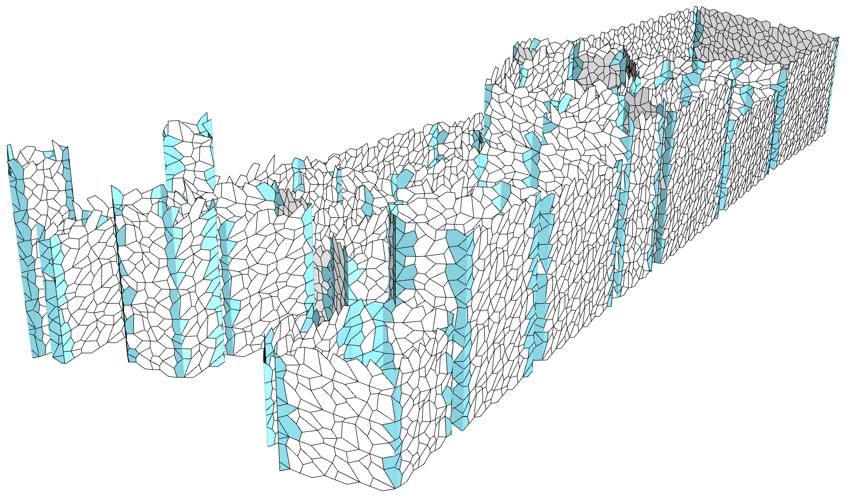
\includegraphics[width=1\textwidth]{Figures/Overview.png}
	\caption{"Voronoi" tiling of KSA Pavilion}
	\label{overview}
\end{figure}

\begin{figure}[hbt!]
	\centering
	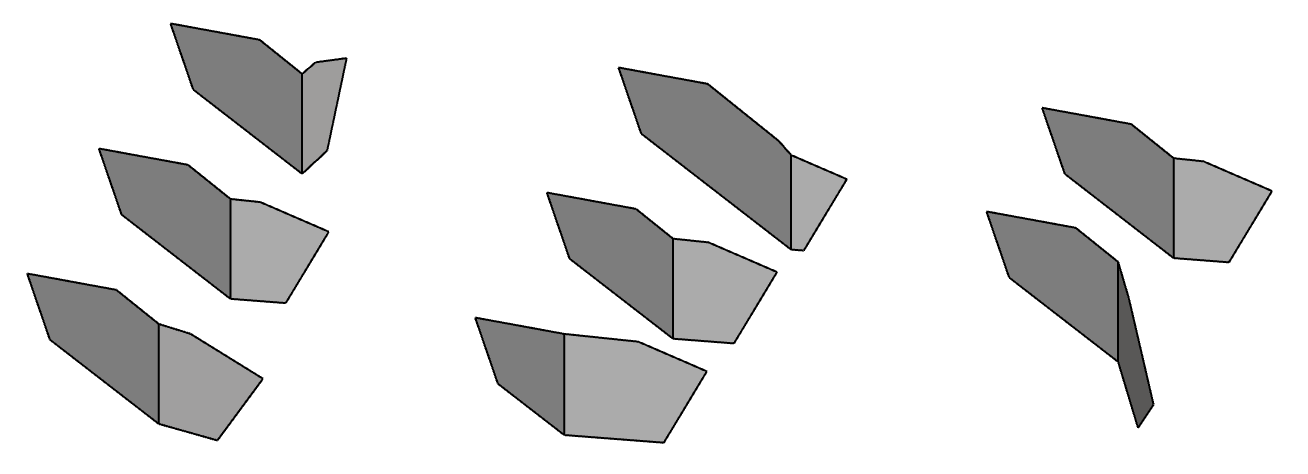
\includegraphics[width=1\textwidth]{Figures/Tiles.png}
	\caption{
        (Left) Different tiles introduced by different angles  
        (Middle) Different tiles introduced by different folding positions  
        (Right) Mirrored tiles are not the same
    }
	\label{tile}
\end{figure}

Through only grasshopper, it is challenging to determine whether two Breps are same. It may involve finding an orienting method and checking the alignments of all vertices, which are slow and complicated especially for categorizing a large number of Breps all consist of multiple surfaces.

Therefore, a fast method is needed where distinct numeric attributes of arbitrary shapes irrelevant to the tiles' orientation are retrieved as unique identifiers. The process to generate identifiers should: \textbf{1) Be deterministic for the same shape} (For example, the process of picking two vertices based on points' distances to other points is not deterministic if applied to a square) \textbf{2) Be different for different shapes} (Examples in Section \ref{Clarification}).

\section{Domain}

The method introduced in this document are applicable to geometries of following characteristics: 1) Consists of one surface or multiple surfaces with shared edges (A single Rhino BRep type geometry); 2) All component surfaces are planar; 3) All edges are straight.

\section{Identifying Arbitrary Shape} \label{IdentifyShape}

\subsection{Steps}

\noindent

Let $V$ and $E$ be the collections of vertices and edges extracted by Grasshopper's \textit{Deconstruct Brep} component.

1. Retrieve a collection of points $P$, i.e. the union of all vertices and midpoints of edges:
\begin{align*}
	P = V \cup \{\text{Midpoint}(e) | e \in E \}
\end{align*}

2. Obtain pairwise distances of $P$:
\begin{gather*}
	D = \{\text{Distance}(P_i, P_j) | 1 \leq i < j \leq |P| \} \\
	(\text{Thus } |D| = \frac{|P|(|P| - 1)}{2})
\end{gather*}

3. Concatenate the sorted sequence of $D$ as the identifier of this shape:
\begin{align*}
	D_{(1)}D_{(2)}...D_{(n)} \text{ where } D_{(1)} < D_{(2)} < ... < D_{(n)}, n = |D|
\end{align*}

\subsection{Examples}

\subsubsection{$1-2-\sqrt{5}$ Triangle} 15 distances will be obtained from a triangle (Figure \ref{idexample1}). Rounding numbers to 3 decimal places, the identifier will be: 
 500\textbf{500}500\textbf{1000}1000\textbf{1000}1000\textbf{1118}1118\textbf{1118}1118\textbf{1414}2000\textbf{2062}2236

\begin{figure}[hbt!]
	\centering
	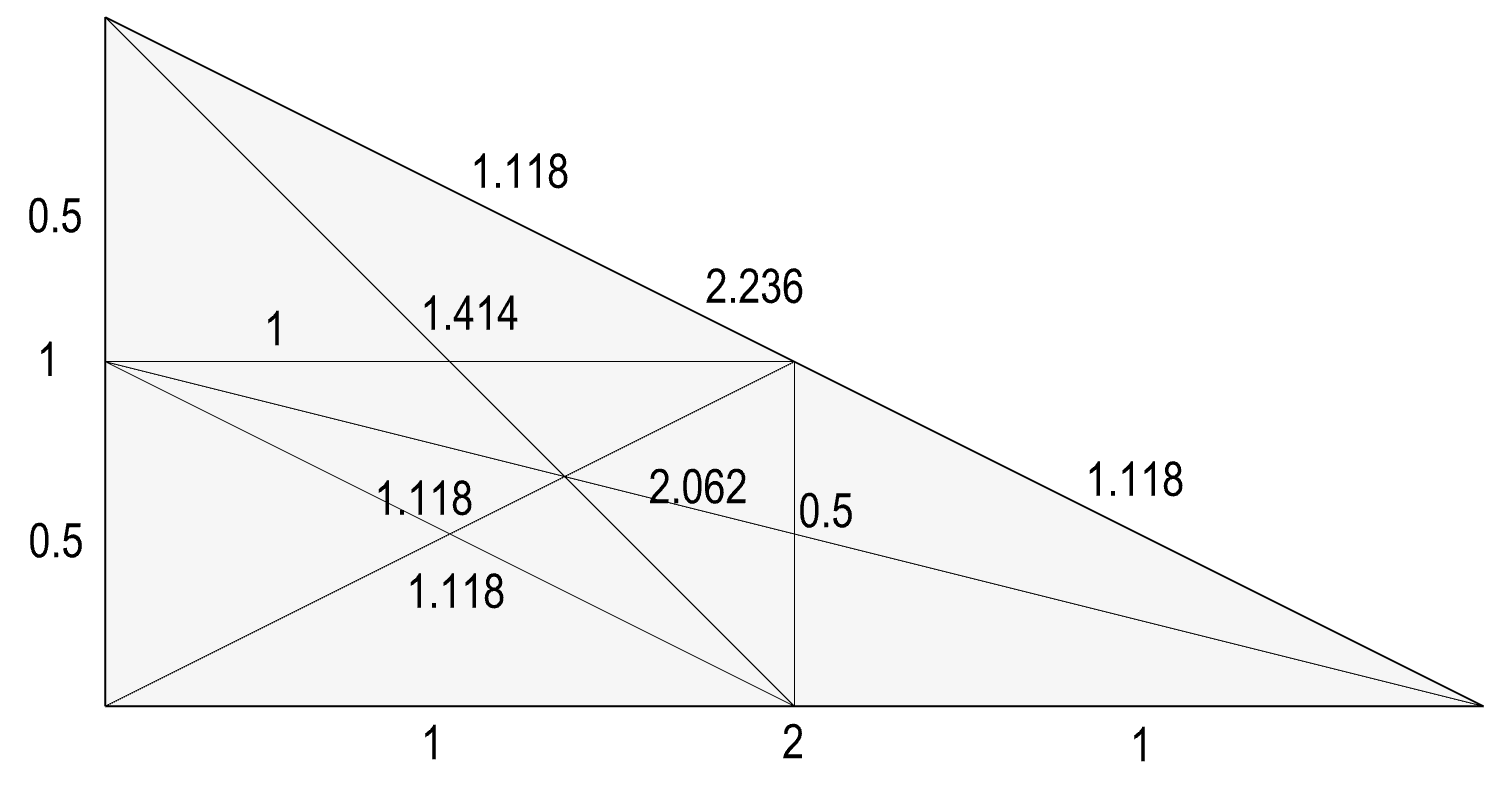
\includegraphics[width=0.6\textwidth]{Figures/IdentifierExample1.png}
	\caption{
        The pairwise distances in an $1-2-\sqrt{5}$ triangle	
    }
	\label{idexample1}
\end{figure}

\subsubsection{Folded Shape} 55 distances will be obtained from a folded shape consists of one triangle and one quadrilateral (Figure \ref{idexample2}). Note that the three dimensional distances across the two components will vary based on the folding angle, which serve as an identifier to the angle.

\begin{figure}[hbt!]
	\centering
	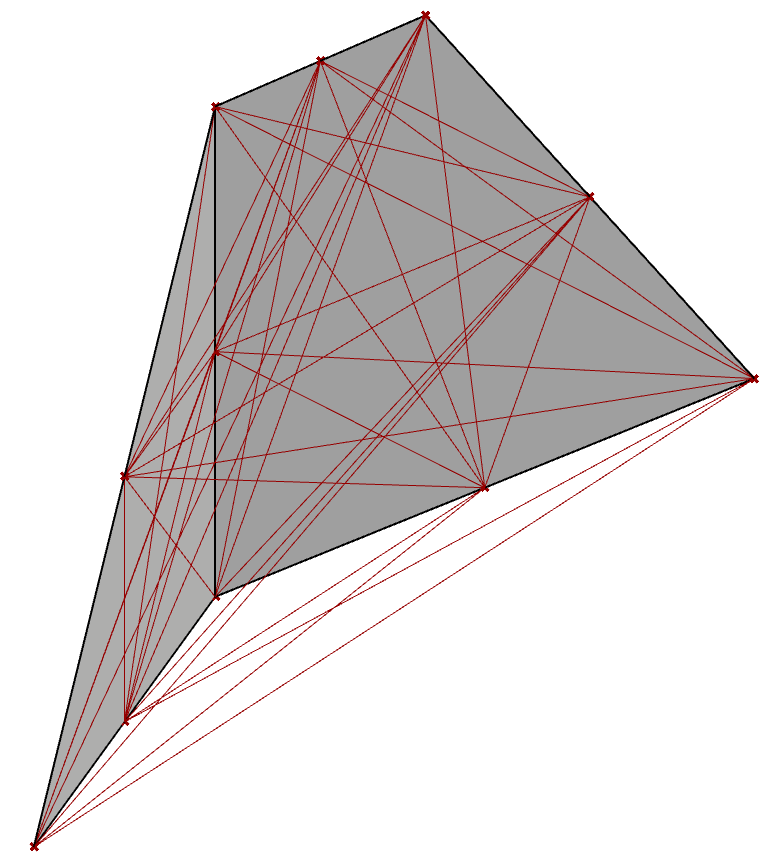
\includegraphics[width=0.25\textwidth]{Figures/IdentifierExample2.png}
	\caption{
        Visualized pairwise distances in a folded shape
    }
	\label{idexample2}
\end{figure}

\FloatBarrier

\subsection{Clarification} \label{Clarification}

\subsubsection{The necessity of including edge midpoints}

Using $P = V$ fails to distinguish the following pair (Figure \ref{idcexample1}):

\begin{figure}[hbt!]
	\centering
	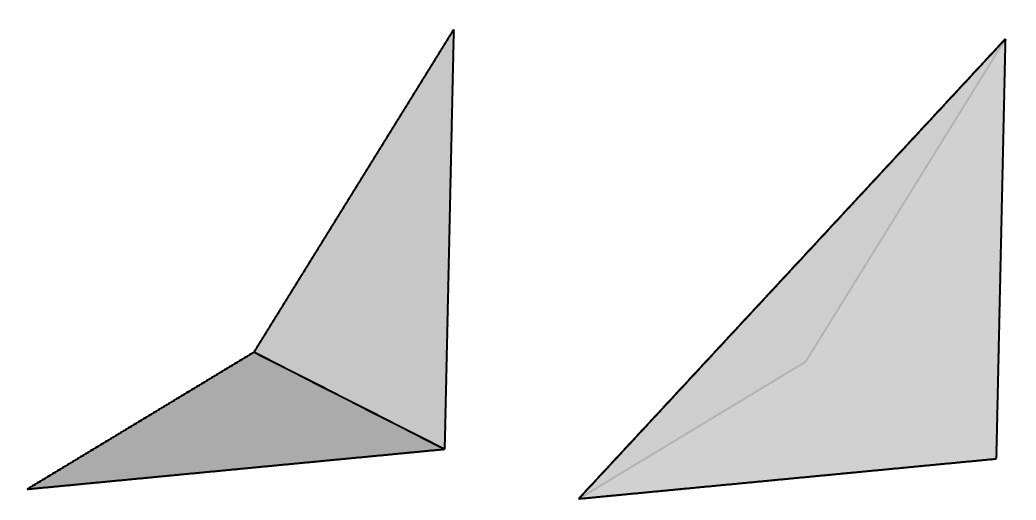
\includegraphics[width=0.5\textwidth]{Figures/IdentifierCounterExample1.png}
	\caption{
        A pair of shapes having the same set of vertices
    }
	\label{idcexample1}
\end{figure}

\subsubsection{The necessity of including vertices}

Using $P = \{\text{Midpoint}(e) | e \in E \}$ fails to distinguish the following pair (Figure \ref{idcexample2}):

\begin{figure}[hbt!]
	\centering
	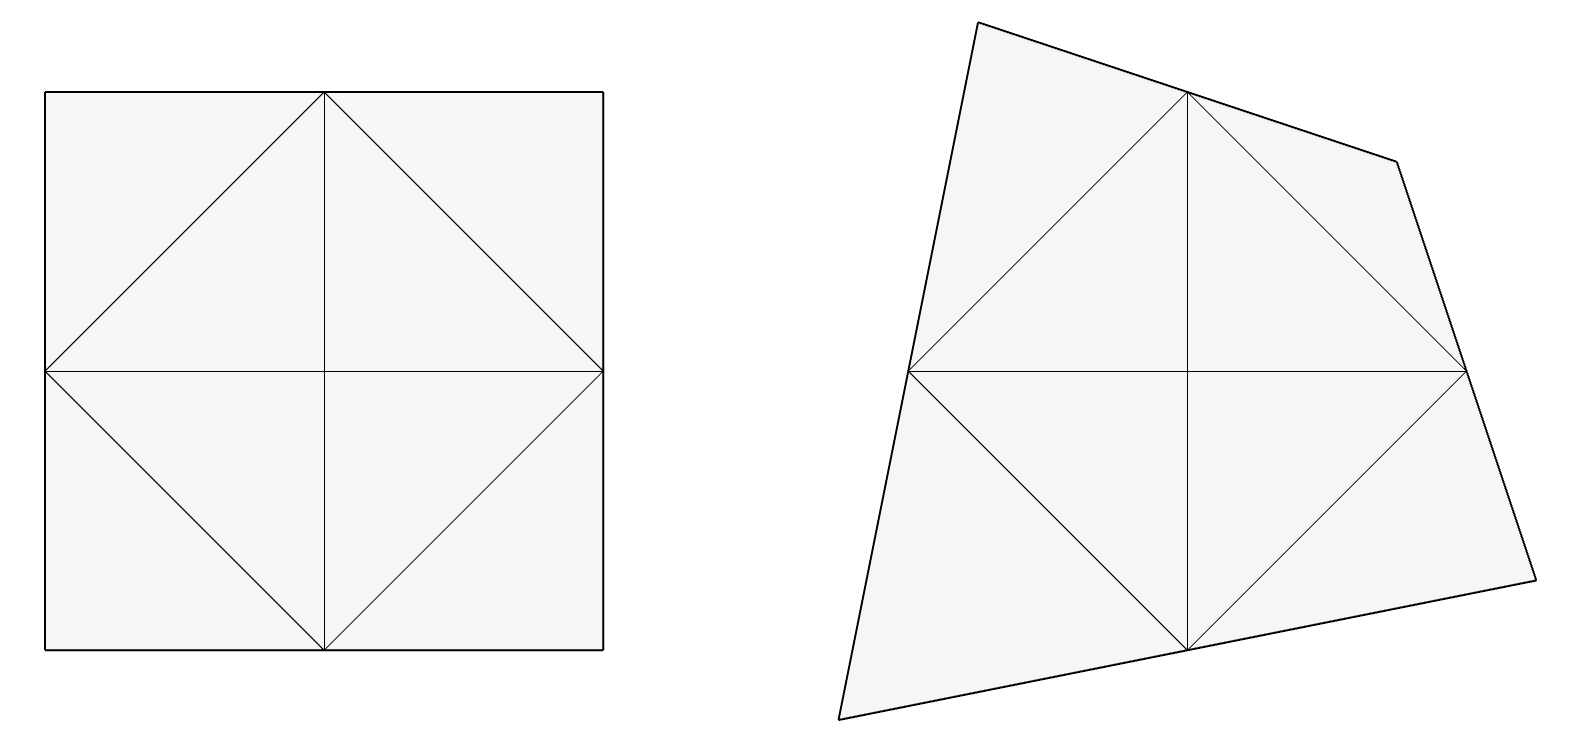
\includegraphics[width=0.5\textwidth]{Figures/IdentifierCounterExample2.png}
	\caption{
        A pair of shapes having the same set of edge midpoints
    }
	\label{idcexample2}
\end{figure}

\section{Distinguishing Mirrored Shapes} \label{IdentifyMirror}

The method described above works for planar shapes, but relative distances will be the same for mirrored non-planar geometry. Therefore, an extra method is developed for distinguishing mirrored geometries consists of multiple non-planar surfaces.

\subsection{Steps}

Use the same method from previous section to retrieve $P$. Let $C$ be the collection of centroids extracted by Grasshopper's \textit{Area} component.

1. Define a function $F$, serving as a generic method to deterministically pick points from a geometry:
\begin{align*}
	F(p) = \sum_{i=1}^{|P|}\text{Distance}(p, P_i)
\end{align*}

2. Obtain three points $P_a, P_b, P_c$:
\begin{align*}
	P_a &= \arg \min_{P_i}F(P_i) \\
	P_b &= \arg \min_{C_i}F(C_i) \\
	P_c &= \arg \max_{C_i}F(C_i)
\end{align*}

3. Obtain two vectors $W_a, W_b$:
\begin{align*}
	\vec{W_a} = P_b - P_a \\
	\vec{W_b} = P_c - P_a
\end{align*}

4. Obtain a position $P^*$:
\begin{align*}
	P^* = P_a + \vec{W_a} \times \vec{W_b}
\end{align*}

If $\arg \min_{C_i}F(C_i) = \arg \max_{C_i}F(C_i)$, obtain two positions $P^*_a, P^*_b$:
\begin{align*}
	P^*_a = P_a + \vec{W_a} \times \vec{W_b} \\
	P^*_b = P_a + \vec{W_b} \times \vec{W_a}
\end{align*}

5. Obtain the distances of all vertices to this position:
\begin{gather*}
	D' = \{\text{Distance}(P_i, P^*) | 1 \leq i \leq |P| \} \\
	(\text{Thus } |D| = |P|) \\
	\text{or} \\
	D' = \{\text{Distance}(P_i, P^*_a), \text{Distance}(P_i, P^*_b) | 1 \leq i \leq |P| \} \\
	(\text{Thus } |D| = 2|P|)
\end{gather*}

6. Concatenate the sorted sequence of $D'$ as the identifier of this shape:
\begin{align*}
	D'_{(1)}D'_{(2)}...D'_{(n)} \text{ where } D'_{(1)} < D'_{(2)} < ... < D'_{(n)}, n = |D'|
\end{align*}

\subsection{Example}

Below is an example where vectors and distances involved in the process are visualized (Figure \ref{idexample3}) for a pair of mirrored geometries. It is clear that their $D'$ are completely different.

\begin{figure}[hbt!]
	\centering
	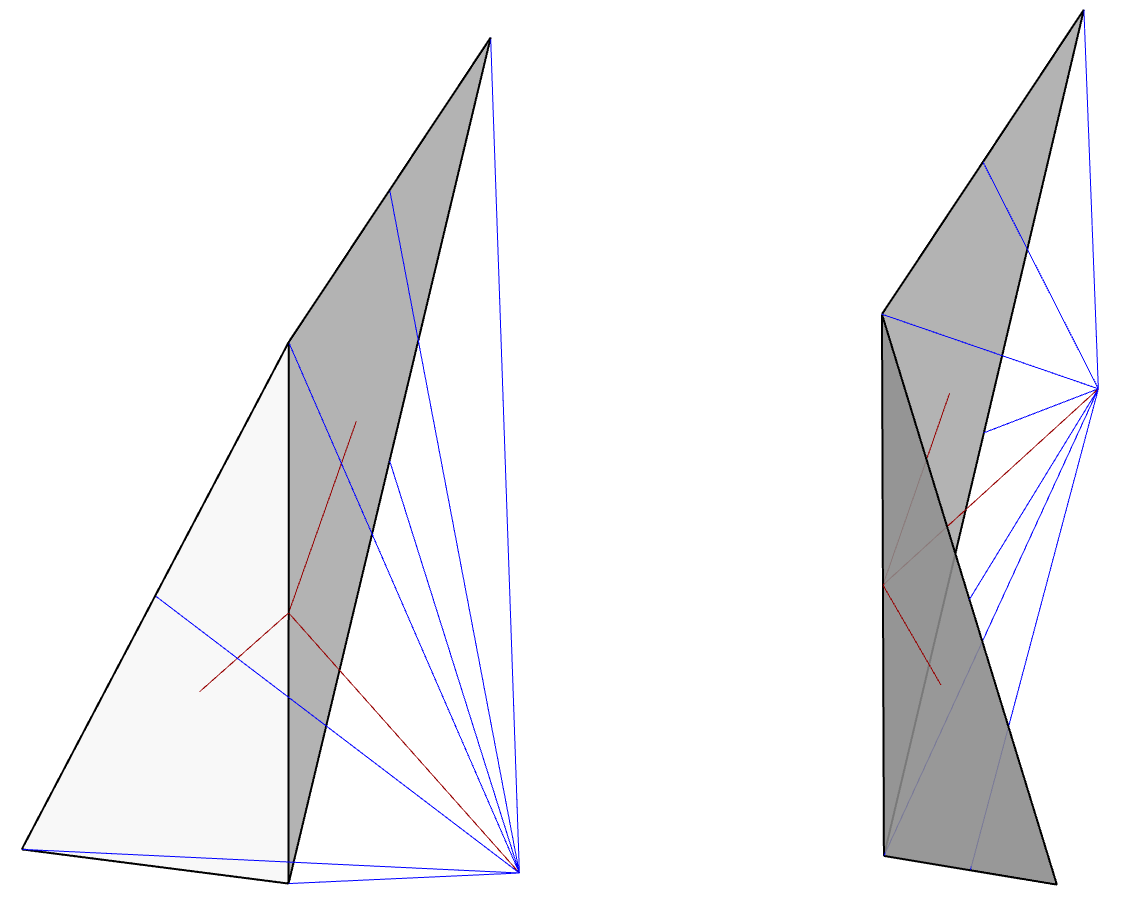
\includegraphics[width=0.5\textwidth]{Figures/IdentifierExample3.png}
	\caption{
        Visualized $W_a, W_b, P_aP^*$ (Red, scaled for demonstration) and $D'$ (Blue) for a pair of mirrored geometries.
    }
	\label{idexample3}
\end{figure}

\FloatBarrier

\subsection{Note}

\subsubsection{Robustness} \label{robustness} Despite of the extra part in step 4, this method may fail if $|\arg \min_{P_i}F(P_i)| > 2$ or $|\arg \min_{C_i}F(C_i)| > 2$ or $|\arg \max_{C_i}F(C_i)| > 2$, i.e. there are multiple equivalent points to pick. See one example below (Figure \ref{idcexample3}). Therefore, this method is more suitable for counting irregular shapes without a high order of symmetry.

\begin{figure}[hbt!]
	\centering
	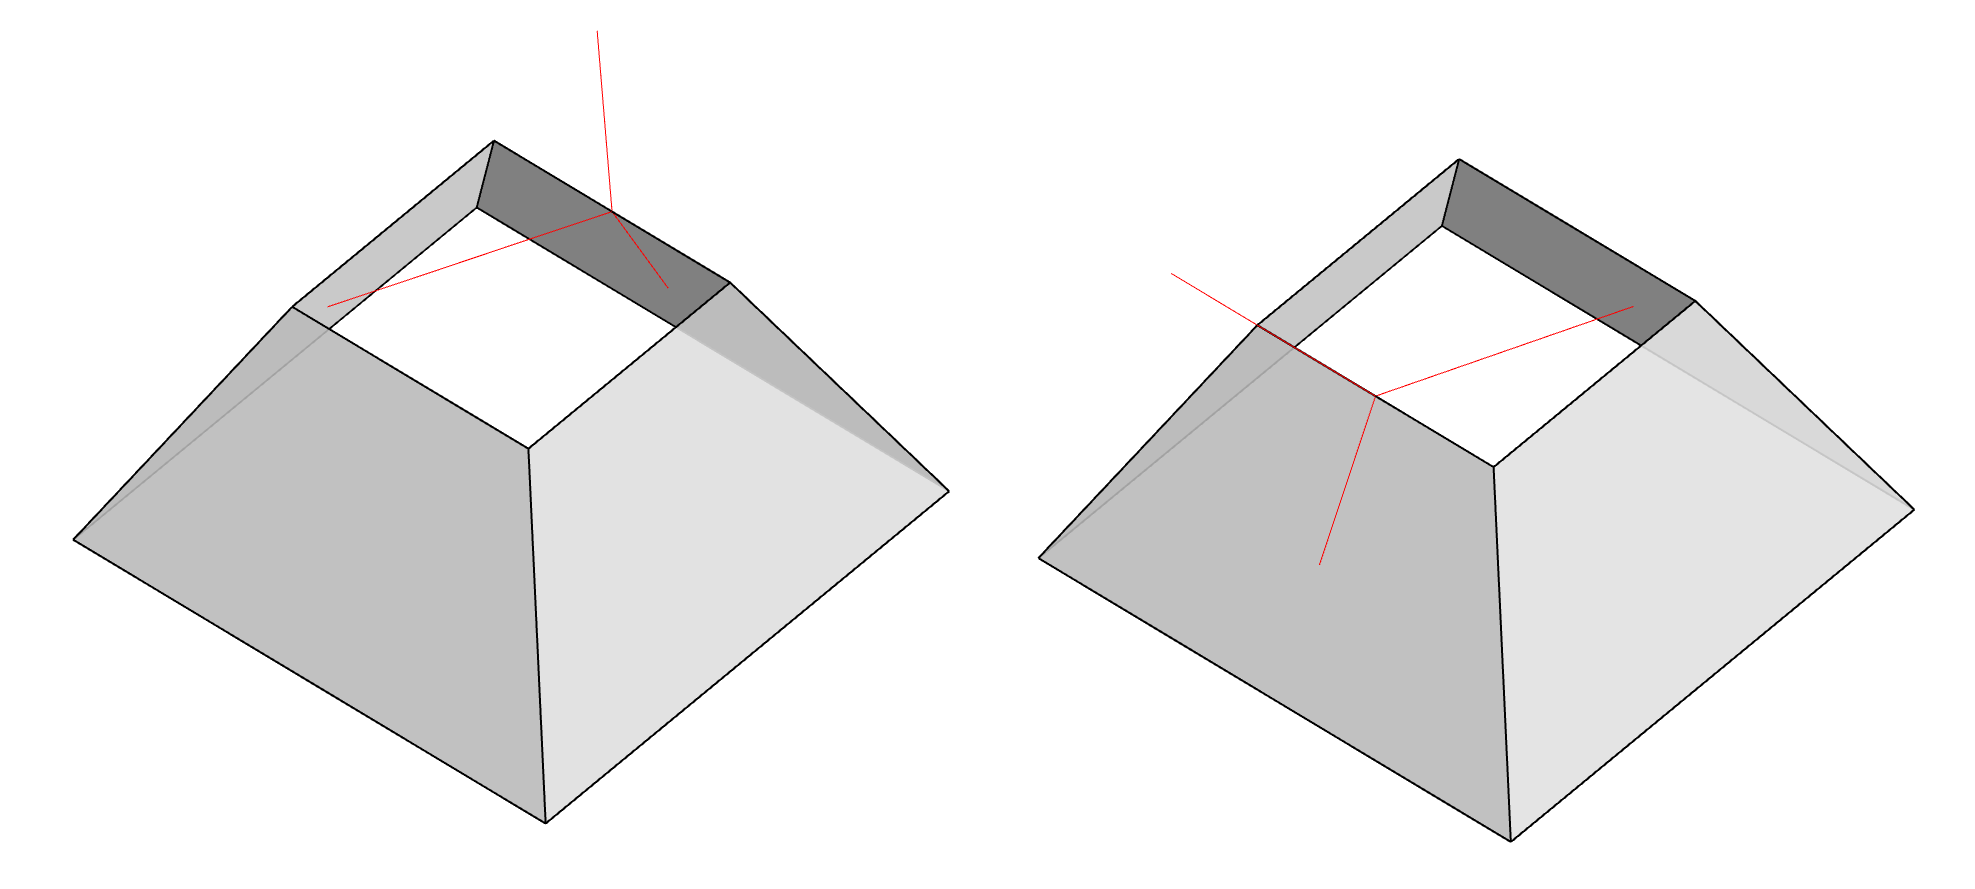
\includegraphics[width=0.8\textwidth]{Figures/IdentifierCounterExample3.png}
	\caption{
        A pair of geometries having multiple equivalent edge midpoints and face centroids, leading to different $P^*$ positions.
    }
	\label{idcexample3}
\end{figure}

\subsubsection{Necessity} In current script, this identifier is append to the previous identifier (Section \ref{IdentifyShape}). However, it is not clear whether this identifier itself is unique for arbitrary non-planar shapes. A general proof or counter example is welcome.

\section{Postprocess}

With identifiers, classes from C\#, for example \href{https://learn.microsoft.com/en-us/dotnet/api/system.collections.generic.hashset-1?view=net-7.0}{HashSet}, are convenient to perform categorization, count number of unique tiles, and query each shape. Optionally, \href{https://learn.microsoft.com/en-us/dotnet/api/system.security.cryptography.sha256?view=net-7.0}{SHA256 algorithm} can be applied to reduce the length of identifiers. (Figure \ref{result})

\begin{figure}[hbt!]
	\centering
	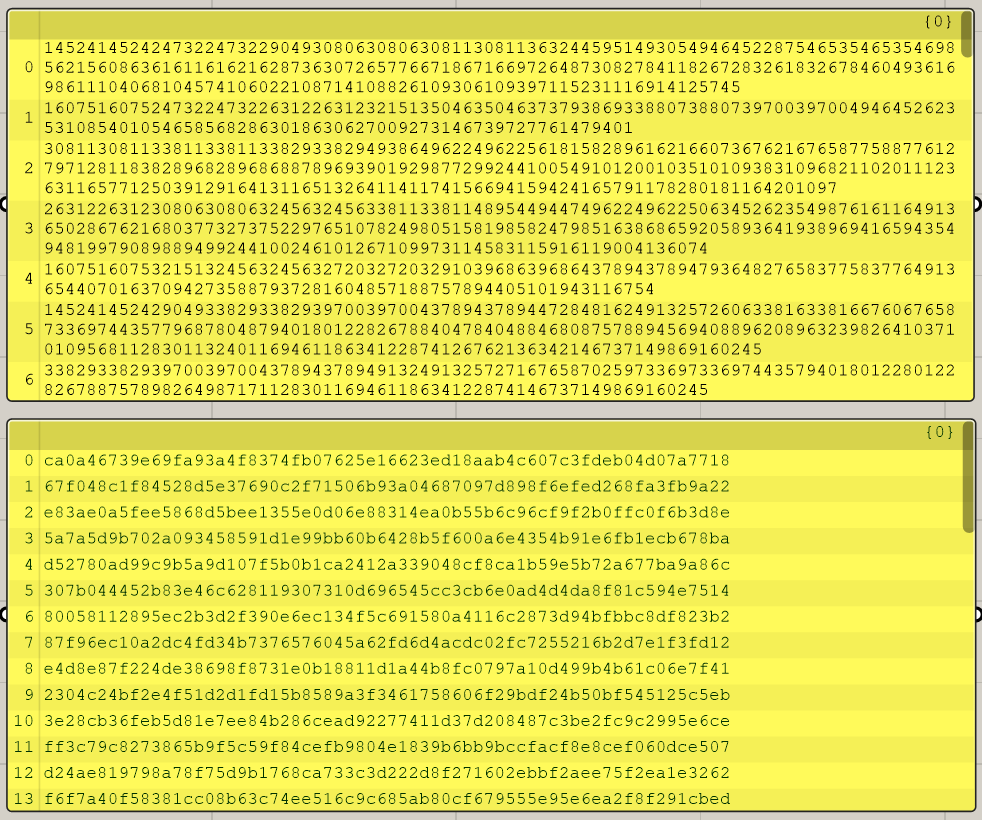
\includegraphics[width=0.8\textwidth]{Figures/EncodedTiles.png}
	\caption{
        Encoded identifiers of tiles for KSA Pavilion (Top) and their SHA256 encoded results (Bottom).
    }
	\label{result}
\end{figure}

\end{document}